\subsection{Interpreter Architecture}

The interpreter operates by inspecting the source instruction at the current program counter (PC) and executing the appropriate C++ code to emulate the behaviour of the source instruction. It then increments the PC and repeats until program execution is complete.

\begin{figure}[h]
    \centering
    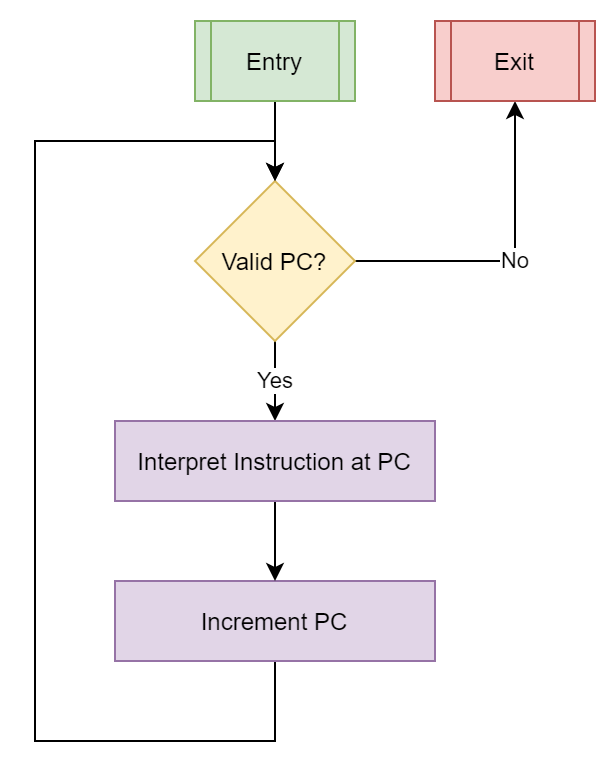
\includegraphics[width=0.5\linewidth]{diagrams/interpreter.png}
    \caption{Top level architecture of the interpreter emulator.}
    \label{figure:interpreter-arch}
\end{figure}

\subsubsection{Interpreter Core}

The core emulator \JW{These subsubsections are very short -- perhaps better as items in a bulleted description list like you had in Section 3.3?} component of the interpreter. It does not control the execution flow but is responsible for interpreting individual instructions. This was separated into its own modular component, so it could be reused in further emulators such as the hybrid emulator.

\subsubsection{Register File}
\label{section:interpreter-reg-file}

The register file models the 32 general purpose registers found in MIPS-1 in addition to the special \texttt{\$hi} and \texttt{\$lo} registers. The register values are stored contiguously for better cache performance. All writes to \texttt{\$0} are ignored, preserving its constant zero value.

\subsubsection{Memory Map}
\label{section:interpreter-mem-map}

The memory map uses an associative model powered by an unordered hash table. This allows for the entire 32-bit address space to be emulated without requiring it to be pre-allocated, something that might prove difficult in a 32 bit process. The current implementation allows for $\mathcal{O}(1)$ read and write times. Despite this, the performance is substandard compared to a raw array due to the extra overhead and being less cache friendly.

After profiling, the \texttt{std::unordered\_map} originally used was found to be a bottleneck and thus was replaced with a 3rd party implementation Tessil/robin-map \cite{tessil-map, tessil-benchmark}. \JW{Cool! Really nice detail to include.}